\label{Chapter:SimCLR}

Until this point of the work, we have been presenting the theoretical basis of representation learning using contrastive learning. Previous approaches, such as  the framework presented in \cite{oord_representation_2019}, use a generative approach as a part of the representation learning process. Although this can be beneficial at some points and, in fact, achieved the \emph{state-of-art}\footnotemark empirical results, we have to consider that generative models have some drawbacks. 

%------------- Footnotemark
\footnotetext{\emph{State-of-art} refers to the best results that have been achieved at some point of time.}
%----------------------


Let us set in the case of learning representations of images to present a very simple example. In this case, generative models must \emph{generate} each pixel on the image. This can be extremely computationally expensive. 

Until now, we had been trying to minimize the loss in Equation \eqref{NCE:loss}, which we proved that maximizes a lower bound in the mutual information. However, some papers such as \cite{chen_simple_2020}, \cite{tschannen_mutual_2020}, suggest that it is unclear if the success of their methods is caused by the maximization of mutual information between the latent representations, or by the specific form that the constrastive loss has.

In fact, in \cite{tschannen_mutual_2020} they provide empirical proof for the loose connection between the success of the methods that use MI maximization and the utility of the MI maximization in practice. They also empirically proof  that the encoder architecture can be more important than the estimator used to determine the MI.

Even with the empirically proved disconnection between MI maximization and representation quality, recent works that have used the loss function defined in Equation \eqref{NCE:loss} have obtained state-of-art results in practice. 

Both SimCLR and BYOL (the framework that we will present later), are examples of \emph{siamese neural networks}. We remark it as a definition since it is important for the later explanation.

\begin{ndef}
A \emph{siamese neural network} is a type of NN architecture that contains (typically) two NNs which have the same configuration, parameters and weights. The parameters are updated the same way across both networks. 
\end{ndef}

These networks are usually used to find the similarity between the inputs by comparing produced feature vectors. They are more robust to class imbalance, nice to an ensemble with the best classifier (since the classifier is built on top of the representation extractors), and learn from semantic similarity.


\section{SimCLR framework}

\emph{SimCLR} \citep{chen_simple_2020} presents a framework that achieved state-of-art results when it was presented in July 2020. It also uses contrastive learning in an specific way that we will present later. 

This framework learns representations by maximizing agreement between examples of the same input obtained by using data augmentation on the input example and a contrastive loss in the latent space. 


\begin{figure}[H]
    \small
        \centering
    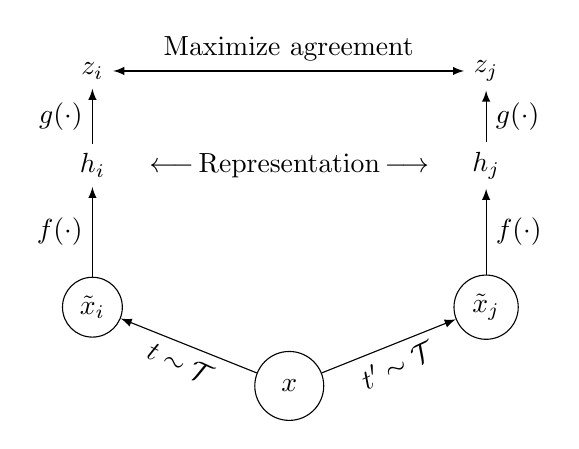
\begin{tikzpicture}
        \node at (0,1.8) (h) {$\longleftarrow\,$Representation$\,\longrightarrow$};
        \node[draw, circle] at (0,-1) (x) {$\,~\bm{x}~\,$};
        \node[draw, circle] at (-2.5,0) (x1) {$\tilde{\bm{x}}_i$};
        \node[draw, circle] at (2.5,0) (x2) {$\tilde{\bm{x}}_j$};
        \node at (-2.5,1.8) (h) {$\bm h_i$};
        \node at (2.5,1.8) (c) {$\bm h_j$};
        \node at (-2.5,3) (hh) {$\bm z_i$};
        \node at (2.5,3) (cc) {$\bm z_j$};
        \path[->] 
            (x)  edge [>=latex] node[below,rotate=-25] {$t\sim\mathcal{T}$} (x1)
            (x)  edge [>=latex] node[below,rotate=25] {$t'\sim \mathcal{T}$} (x2)
            (x1)  edge [>=latex] node[left,rotate=0] {$f(\cdot)$} (h)
            (x2)  edge [>=latex] node[right,rotate=0] {$f(\cdot)$} (c)
            (h)  edge [>=latex] node[left,rotate=0] {$g(\cdot)$} (hh)
            (c)  edge [>=latex] node[right,rotate=0] {$g(\cdot)$} (cc);
        \path[<->]
            (hh)  edge [>=latex] node[above,rotate=0] {Maximize agreement} (cc);
        \end{tikzpicture}
        \caption{Figure obtained from \cite{chen_simple_2020}. A simple framework for contrastive learning of visual representations.}
        \label{fig:framework:SimCLR}
    \end{figure}


The framework that is presented follows a linear structure. Figure \ref{fig:framework:SimCLR} depicts it. Let us provide with deeper explanation. We will present the steps in a general way and later we will remark the specific considerations that were used in the implementation of the framework for the experiments. 

The steps followed are:
\begin{enumerate}
\item Firstly, using the input $x$ and two augmentation functions $t,t' \in \mathcal T$, two different views $\tilde x_i,\tilde x_j$ are obtained using data augmentation. They are both sampled from the same family of data augmentations $\mathcal T$. They are \emph{both} considered as positive views.
\item Secondly, a NN base encoder $f(\cdot)$ is used to extract representations for the two different views, obtaining $h_i = f(\tilde{x_i})$, where $h_i \in \R^d$.  

\item Then, a \emph{small} neural network projection $g(\cdot)$ is used. This neural network maps the representations $h_i$ to the space where contrastive loss is applied. Hence, we obtain 
$$
z_i = g(h_i) = W^{(2)}\sigma(W^{(1)}h_i),$$
where $\sigma$ is a nonlinear function and $W^{(i)}$ are the weights matrix.

\item Lastly, the contrastive loss is used for a contrastive prediction task. Using a set $\{\tilde x_k \}$ that includes a pair of positive examples $\tilde x_i,\tilde x_j$, the contrastive loss will (as we have already been doing theoretically) try to identify $\tilde x_j$ in the set for a given $\tilde x_i$. It is important to remark how the contrastive loss is used in this framework:
\begin{enumerate}
\item A minibatch of $N$ samples is randomly taken from the training set. 
\item Using the $N$ samples, we augment each pair to obtain $2N$ data points. The idea is, given a positive pair, use the other $2(N-1)$ as negative examples.
\item We define
\[
sim(u,v) = \frac{u^T v}{\norm{u}\norm{v}},    
\]
the normalized dot product between $u$ and $v$. This function is also known as the \emph{cosine similarity}. Then, the loss function for a positive pair of examples takes the form:
\begin{equation}\label{c:loss:simclr:ind}
\ell_{i,j} = -\log \frac{exp(sim(z_i,z_j)/\tau)}{\sum_{k=1}^{2N} \mathbb{1}_{k \neq i} exp(sim(z_i,z_k)/\tau)},    
\end{equation}
where $\mathbb{1}_{k \neq i} \in \{0,1\}$ produces $0$ if $k = i$ and $1$ elsewhere. $\tau$ is a temperature parameter that has to be adjusted.
\item The final loss is computed across all the positive pairs, both $(i,j)$ and $(j,i)$ in the minibatch.
\begin{equation}\label{c:loss:simclr}
\mathcal L = \frac{1}{2N} \sum_{k=1}^{2N} \left(\ell(2k-1,2k) + \ell(2k,2k-1)\right).
\end{equation}
\end{enumerate}
\end{enumerate}
\begin{remark}
The loss in Equation \eqref{c:loss:simclr} is just another formulation of the one in Equation \eqref{NCE:loss}, applied to this particular way of obtaining positive and negative views.
\end{remark}

We can summarize all this steps in the following algorithm:
\begin{figure}[H]
\begin{algorithm}[H]
    \caption{\label{alg:main} SimCLR's learning algorithm.}
    \begin{algorithmic}
        \STATE \textbf{input:} batch size $N$, temperature $\tau$, structure of $f$, $g$, $\mathcal{T}$.
        \FOR{sampled minibatch $\{\bm x_k\}_{k=1}^N$}
        \STATE \textbf{for all} $k\in \{1, \ldots, N\}$ \textbf{do}
            \STATE $~~~~$draw two augmentation functions $t \!\sim\! \mathcal{T}$, $t' \!\sim\! \mathcal{T}$
            \STATE $~~~~$\textcolor{gray}{\# use augmentations} 
            \STATE $~~~~$$\tilde{\bm x}_{2k-1} = t(\bm x_k)$
            \STATE $~~~~$$\tilde{\bm x}_{2k} = t'(\bm x_k)$
            \STATE $~~~~$\textcolor{gray}{\# use $f$} 
            \STATE $~~~~$$\bm h_{2k-1} = f(\tilde{\bm x}_{2k-1})$  \textcolor{gray}{~~~~~~~~~~~~~~~~~~~~~~~~~~~~~~\# representation}
            \STATE $~~~~$$\bm h_{2k} = f(\tilde{\bm x}_{2k})$      \textcolor{gray}{~~~~~~~~~~~~~~~~~~~~~~~~~~~~~~~~~~~~~~\# representation}
            \STATE $~~~~$\textcolor{gray}{\# use $g$} 
            \STATE $~~~~$$\bm z_{2k-1} = g({\bm h}_{2k-1})$  \textcolor{gray}{~~~~~~~~~~~~~~~~~~~~~~~~~~~~~~~~\# projection}
            \STATE $~~~~$$\bm z_{2k} = g({\bm h}_{2k})$      \textcolor{gray}{~~~~~~~~~~~~~~~~~~~~~~~~~~~~~~~~~~~~~~~~\# projection}
        \STATE \textbf{end for}
        \STATE \textbf{for all} $i\in\{1, \ldots, 2N\}$ and $j\in\{1, \dots, 2N\}$ \textbf{do}
        \STATE $~~~~$ $s_{i,j} = \bm z_i^\top \bm z_j / (\lVert\bm z_i\rVert \lVert\bm z_j\rVert)$ \textcolor{gray}{~~~~~~~~\# compute similarity}\\
        \STATE \textbf{end for}
        \STATE update networks $f$ and $g$ to minimize $\mathcal{L}$ defined in Eq. \eqref{c:loss:simclr}
        \ENDFOR
        \STATE \textbf{return} encoder network $f(\cdot)$, and throw away $g(\cdot)$
    \end{algorithmic}
    \end{algorithm}
    
    \caption{Algorithm that summarizes the learning process that SimCLR follows.}
\end{figure}

Considerations:
\begin{enumerate}
\item In SimCLR, the data augmentation is applied sequentially, and using three techniques of image data augmentation that are very simple and common:
\begin{enumerate}
\item Random cropping followed by resize to original size,
\item Random color distortions, which consist of changing the value of certain amount of pixels randomly, like color jittering or changing from colored images to black and white images.
\item Random Gaussian Blur: Gaussian Blur consists of convolving an image with a \emph{Gaussian function}.
\end{enumerate}

\item For the base encoder $f(\cdot)$, a \emph{ResNet} network is used because of its simplicity.
\item For the projection head $g(\cdot)$, a MLP with one hidden layer is used, and \emph{ReLU} is used as the activation function $\sigma$.
\end{enumerate}



\section{Findings of SimCLR}

    Using the algorithm structure that we have presented, the experiments focused on finding what made the biggest impact on the representation learning task. 
    
    Intuitively, since we are comparing $2N$ images, either positive or negative, the batch size that we will use for the experiment should be as big as possible. Comparing a positive sample and trying to push it apart from as much negative samples as possible in the same iteration sounds like a good idea for the quality of our representations.
    
    
    A few of the most relevant findings using SimCLR are: 
    \begin{itemize}
    \item In the SimCLR framework, multiple data augmentations are used and it is empirically shown that this improves the contrastive prediction tasks that yield effective representations.
    
    \item The introduction of a nonlinear transformation that it can be learnt during the learning process. This linear transformation is between the representation and the contrastive loss, so before evaluating the loss function, the representation is applied the nonlinear function.
    
    \item The contrastive loss benefits from normalized embeddings and also from a temperature parameter that has to be adjusted.
    
    \item This loss also benefits from larger batch sizes and longer training, as well as from deeper and wider networks.
\end{itemize}

Later, \emph{SimCLRv2} was presented \citep{chen2020big}, achieving a new state-of-art in semi-supervised learning on the ImageNet dataset. In this new framework, semi-supervised learning is use . This approach involves unsupervised learning followed by supervised fine-tuning\footnotemark. After this stages that are similar to SimCLR,  a final stage is added. It consists of \emph{distillation} with unlabeled examples for refining the task-specific knowledge.


In the self-supervised (or unsupervised) part, the images are used without its labels, so that the representations of them that are obtained by the framework are not related to an specific task. Using this technique, \cite{chen2020big} shows how using deeper and wider neural networks for both self-supervised pretraining and fine-tuning improves accuracy greatly. Also, the importance of the projection head $g(\cdot)$ is remarked in this new framework.
%------------- Footnotemark
\footnotetext{\emph{Fine-Tuning} refers to the process of re-training certain parts of an already trained NN so that it focuses its learn on specific examples, such as a different dataset.}
%----------------------